\documentclass[12pt,twoside]{article}
\usepackage[dvipsnames]{xcolor}
\usepackage{tikz,graphicx,amsmath,amsfonts,amscd,amssymb,bm,cite,epsfig,epsf,url}
\usepackage[hang,flushmargin]{footmisc}
\usepackage[colorlinks=true,urlcolor=blue,citecolor=blue]{hyperref}
\usepackage{amsthm,multirow,wasysym,appendix}
\usepackage{array,subcaption} 
% \usepackage[small,bf]{caption}
\usepackage{bbm}
\usepackage{pgfplots}
\usetikzlibrary{spy}
\usepgfplotslibrary{external}
\usepgfplotslibrary{fillbetween}
\usetikzlibrary{arrows,automata}
\usepackage{thmtools}
\usepackage{blkarray} 
\usepackage{textcomp}
\usepackage[left=0.8in,right=1.0in,top=1.0in,bottom=1.0in]{geometry}

%% Probability operators and functions
%
% \def \P{\mathrm{P}}
\def \P{\mathrm{P}}
\def \E{\mathrm{E}}
\def \Var{\mathrm{Var}}
\let\var\Var
\def \Cov {\mathrm{Cov}} \let\cov\Cov
\def \MSE {\mathrm{MSE}} \let\mse\MSE
\def \sgn {\mathrm{sgn}}
\def \R {\mathbb{R}}
\def \C {\mathbb{C}}
\def \N {\mathbb{N}}
\def \Z {\mathbb{Z}}
\def \cV {\mathcal{V}}
\def \cS {\mathcal{S}}

\newcommand{\RR}{\ensuremath{\mathbb{R}}}

\DeclareMathOperator*{\argmin}{arg\,min}
\DeclareMathOperator*{\argmax}{arg\,max}
\newcommand{\red}[1]{\textcolor{red}{#1}}
\newcommand{\blue}[1]{\textcolor{blue}{#1}}
\newcommand{\green}[1]{\textcolor{ForestGreen}{ #1}}
\newcommand{\fuchsia}[1]{\textcolor{RoyalPurple}{ #1}}



%
%% Probability distributions
%
%\def \Bern    {\mathrm{Bern}}
%\def \Binom   {\mathrm{Binom}}
%\def \Exp     {\mathrm{Exp}}
%\def \Geom    {\mathrm{Geom}}
% \def \Norm    {\mathcal{N}}
%\def \Poisson {\mathrm{Poisson}}
%\def \Unif    {\mathrm {U}}
%
\DeclareMathOperator{\Norm}{\mathcal{N}}

\newcommand{\bdb}[1]{\textcolor{red}{#1}}

\newcommand{\ml}[1]{\mathcal{ #1 } }
\newcommand{\wh}[1]{\widehat{ #1 } }
\newcommand{\wt}[1]{\widetilde{ #1 } }
\newcommand{\conj}[1]{\overline{ #1 } }
\newcommand{\rnd}[1]{\tilde{ #1 } }
\newcommand{\rv}[1]{ \rnd{ #1}  }
\newcommand{\rM}{\rnd{ m}  }
\newcommand{\rx}{\rnd{ x}  }
\newcommand{\ry}{\rnd{ y}  }
\newcommand{\rz}{\rnd{ z}  }
\newcommand{\ra}{\rnd{ a}  }
\newcommand{\rb}{\rnd{ b}  }
\newcommand{\rt}{\rnd{ t}  }
\newcommand{\rs}{\rnd{ s}  }


\newcommand{\rpc}{\widetilde{ pc}  }
\newcommand{\rndvec}[1]{\vec{\rnd{#1}}}

\def \cnd {\, | \,}
\def \Id { I }
\def \J {\mathbf{1}\mathbf{1}^T}

\newcommand{\op}[1]{\operatorname{#1}}
\newcommand{\setdef}[2]{ := \keys{ #1 \; | \; #2 } }
\newcommand{\set}[2]{ \keys{ #1 \; | \; #2 } }
\newcommand{\sign}[1]{\op{sign}\left( #1 \right) }
\newcommand{\trace}[1]{\op{tr}\left( #1 \right) }
\newcommand{\tr}[1]{\op{tr}\left( #1 \right) }
\newcommand{\inv}[1]{\left( #1 \right)^{-1} }
\newcommand{\abs}[1]{\left| #1 \right|}
\newcommand{\sabs}[1]{| #1 |}
\newcommand{\keys}[1]{\left\{ #1 \right\}}
\newcommand{\sqbr}[1]{\left[ #1 \right]}
\newcommand{\sbrac}[1]{ ( #1 ) }
\newcommand{\brac}[1]{\left( #1 \right) }
\newcommand{\bbrac}[1]{\big( #1 \big) }
\newcommand{\Bbrac}[1]{\Big( #1 \Big)}
\newcommand{\BBbrac}[1]{\BIG( #1 \Big)}
\newcommand{\MAT}[1]{\begin{bmatrix} #1 \end{bmatrix}}
\newcommand{\sMAT}[1]{\left(\begin{smallmatrix} #1 \end{smallmatrix}\right)}
\newcommand{\sMATn}[1]{\begin{smallmatrix} #1 \end{smallmatrix}}
\newcommand{\PROD}[2]{\left \langle #1, #2\right \rangle}
\newcommand{\PRODs}[2]{\langle #1, #2 \rangle}
\newcommand{\der}[2]{\frac{\text{d}#2}{\text{d}#1}}
\newcommand{\pder}[2]{\frac{\partial#2}{\partial#1}}
\newcommand{\derTwo}[2]{\frac{\text{d}^2#2}{\text{d}#1^2}}
\newcommand{\ceil}[1]{\lceil #1 \rceil}
\newcommand{\Imag}[1]{\op{Im}\brac{ #1 }}
\newcommand{\Real}[1]{\op{Re}\brac{ #1 }}
\newcommand{\norm}[1]{\left|\left| #1 \right|\right| }
\newcommand{\norms}[1]{ \| #1 \|  }
\newcommand{\normProd}[1]{\left|\left| #1 \right|\right| _{\PROD{\cdot}{\cdot}} }
\newcommand{\normTwo}[1]{\left|\left| #1 \right|\right| _{2} }
\newcommand{\normTwos}[1]{ \| #1  \| _{2} }
\newcommand{\normZero}[1]{\left|\left| #1 \right|\right| _{0} }
\newcommand{\normTV}[1]{\left|\left| #1 \right|\right|  _{ \op{TV}  } }% _{\op{c} \ell_1} }
\newcommand{\normOne}[1]{\left|\left| #1 \right|\right| _{1} }
\newcommand{\normOnes}[1]{\| #1 \| _{1} }
\newcommand{\normOneTwo}[1]{\left|\left| #1 \right|\right| _{1,2} }
\newcommand{\normF}[1]{\left|\left| #1 \right|\right| _{\op{F}} }
\newcommand{\normLTwo}[1]{\left|\left| #1 \right|\right| _{\ml{L}_2} }
\newcommand{\normNuc}[1]{\left|\left| #1 \right|\right| _{\ast} }
\newcommand{\normOp}[1]{\left|\left| #1 \right|\right|  }
\newcommand{\normInf}[1]{\left|\left| #1 \right|\right| _{\infty}  }
\newcommand{\proj}[1]{\mathcal{P}_{#1} \, }
\newcommand{\diff}[1]{ \, \text{d}#1 }
\newcommand{\vc}[1]{\boldsymbol{\vec{#1}}}
\newcommand{\rc}[1]{\boldsymbol{#1}}
\newcommand{\vx}{\vec{x}}
\newcommand{\vy}{\vec{y}}
\newcommand{\vz}{\vec{z}}
\newcommand{\vu}{\vec{u}}
\newcommand{\vv}{\vec{v}}
\newcommand{\vb}{\vec{\beta}}
\newcommand{\va}{\vec{\alpha}}
\newcommand{\vaa}{\vec{a}}
\newcommand{\vbb}{\vec{b}}
\newcommand{\vg}{\vec{g}}
\newcommand{\vw}{\vec{w}}
\newcommand{\vh}{\vec{h}}
\newcommand{\vbeta}{\vec{\beta}}
\newcommand{\valpha}{\vec{\alpha}}
\newcommand{\vgamma}{\vec{\gamma}}
\newcommand{\veta}{\vec{\eta}}
\newcommand{\vnu}{\vec{\nu}}
\newcommand{\rw}{\rnd{w}}
\newcommand{\rvnu}{\vc{\nu}}
\newcommand{\rvv}{\rndvec{v}}
\newcommand{\rvw}{\rndvec{w}}
\newcommand{\rvx}{\rndvec{x}}
\newcommand{\rvy}{\rndvec{y}}
\newcommand{\rvz}{\rndvec{z}}
\newcommand{\rvX}{\rndvec{X}}


\newtheorem{theorem}{Theorem}[section]
% \declaretheorem[style=plain,qed=$\square$]{theorem}
\newtheorem{corollary}[theorem]{Corollary}
\newtheorem{definition}[theorem]{Definition}
\newtheorem{lemma}[theorem]{Lemma}
\newtheorem{remark}[theorem]{Remark}
\newtheorem{algorithm}[theorem]{Algorithm}

% \theoremstyle{definition}
%\newtheorem{example}[proof]{Example}
\declaretheorem[style=definition,qed=$\triangle$,sibling=definition]{example}
\declaretheorem[style=definition,qed=$\bigcirc$,sibling=definition]{application}

%
%% Typographic tweaks and miscellaneous
%\newcommand{\sfrac}[2]{\mbox{\small$\displaystyle\frac{#1}{#2}$}}
%\newcommand{\suchthat}{\kern0.1em{:}\kern0.3em}
%\newcommand{\qqquad}{\kern3em}
%\newcommand{\cond}{\,|\,}
%\def\Matlab{\textsc{Matlab}}
%\newcommand{\displayskip}[1]{\abovedisplayskip #1\belowdisplayskip #1}
%\newcommand{\term}[1]{\emph{#1}}
%\renewcommand{\implies}{\;\Rightarrow\;}



\begin{document}

\begin{center}
{\large{\textbf{Homework 1}} } \vspace{0.2cm}\\
Due September 19 at 11 pm
\\
\end{center}
Name: Giulio Duregon

\break

\begin{enumerate}

\item (True or False)
Prove the following statements or provide a counterexample. Let $A$, $B$, and $C$ be events in a probability space.

\begin{enumerate}
\item If $A$ and $B$ are independent, then so are $A^c$ and $B$.
\subitem
\textbf{This is true. Proof as follows:}\\
$
    P(A|B) = P(A) \text{ A and B are independent therefore} \\
    -P(A|B) = -P(A) \text{ Make negative}\\
    1-P(A|B) = 1-P(A) \text{ Add 1 to each side} \\
    P(A^c|B) = P(A^c) \text{ By definition of complements}
$ \\
Here we showed that knowing B does not give us any more information for $A^c$, therefore the two events are independent. 

\item If $A$ and $B$ are conditionally independent given $C$, then they are also conditionally independent given $C^c$.
\subitem
\textbf{This statement is false by counterexample:}\\
Let A,B,C be the following events for two coinflips:\\
A) The first flip is heads \\
B) At least one coinflip is heads \\
C) The second coinflip is heads \\
\par
In these sequence of events, given C, A and B are conditionally independent. This is true because if we know the event C and the event B (atleast one coinflip was heads and the second coinflip was heads) no new information about the first coinflip is derived:
$$P(A|C|B) = P(A) $$
However, if we have $C^c$ then A and B are conditionally dependent. Imagine we know that the second coinflip was not heads ($C^c$), but we also know that event B happened, that at least one of the flips is heads is true. Therefore, we know event A must have happened, that the first coinflip must be heads. Therefore: 
$$P(A|B|C^c) = 1 $$


\item Events in a partition cannot be independent (assume that every event in the partition has nonzero probability). 
\subitem
\textbf{This statement is true} as by definition events in a partition are disjoint. If two events are disjoint, they must be dependent, as we know if one happens then the other does not.

\break

%Two events $A$ and $B$ cannot be both disjoint and independent, unless one of them has probability zero.
\item If $\P\brac{A | B} = 1$ then $\P\brac{B^c | A^c} = 1$. \textbf{This is a true statement, proof as follows} \\

$
P(B^c|A^c) = 1 \text{ Lets manipulate the left side expression and forget the right term for now}$ \\

$ 
 \frac{P(B^c|A^c)}{P(A^c)} = 1 \text{ By conditional probability}
$\\

$
\frac{P((B \cup A)^c)}{1-P(A)} = 1 \text{ By definition of complements}
$\\

$
\frac{1-P(B) - P(A) + P(A\cap B) }{1-P(A)} = 1 \text{ By definition of complements and union of probabilities}$\\

$
    \frac{1-P(A)}{1-P(A)} + \frac{P(A|B)P(B)-P(B)}{1-P(A)} = 1 \text{ Separate out 1-P(A) term, use conditional probability}
$ \\

$
1 + \frac{P(B)\times (P(A|B)-1)}{1-P(A)}= 1 \text{ Factor out P(B)}
$\\

$
1 + \frac{P(B)\times (0}{1-P(A)}= 1 \text{ We are given P(A|B)=1 and our proof is done}
$\\

$
 1 = 1 
$

\item $\P\brac{B | A\cup B} \geq \P\brac{B | A} $. \textbf{This is a true statement, proof as follows}
\subitem
$
    \frac{P(B|A\cup B)}{P(B)} \geq P(B|A)
$\\

$
    \frac{P(B|A\cup B)}{P(A\cup B)} \geq P(B|A) \text{ By conditional probability}
$\\

$
    {P(B)} \geq P(B|A) \times P(B\cup A) \text{ Multiply both sides by P(B union A)}
$\\

$
    {P(B)} \geq P(B|A) \times [P(A) + P(B) - P(A\cap B)] \text{ Expand P(B union A)}
$\\

$
    {P(B)} \geq P(B|A) \times P(A) + P(B|A) \times P(B) - P(B|A) \times P(A\cap B) \text{ Distribute terms}
$\\

$
    {P(B)}-P(B|A)P(B) \geq P(A\cap B) - P(B|A) \times P(A\cap B) \text{ conditional def., subtract P(B|A)P(B)}
$\\

$
    P(B)[1 - P(B|A)] \geq P(A\cap B)[1  - P(B|A)]  \text{ factor like terms}
$\\

$
    P(B) \geq P(A\cap B) \text{ Divide both sides by [1  - P(B|A)]  and we're done}
$\\







\end{enumerate}


\break

\item (Probability spaces)
 

\subitem
\textbf{To prove that we have a valid probability measure}:\\

1) That all probabilities are non negative and no greater than 1 $P(X=x) = 0<= x <=1$\\

We know this is true as our sample space is $\Omega _A$ which contains the collection of events $\ml{F}_A$. The events in $\ml{F}_A$ are the intersection between any event in the sample space $\Omega$ and $A$. We know by virtue of the problem statement that $P(A) \neq 0$, therefore any events in $\ml{F}_A$ will have non-negative probabilities that are also no greater than 1.\\

2) The sum of the space is 1 \\

We know this is true because when we defined our sample space $\Omega _A$ we normalized it by $P(A)$. If we added all the disjoint events in $\ml{F}_A$ that belong to $\Omega _A$, we will sum to 1. \\

3) The union of two disjoint events are the sum of the two events.\\

If $P(A\cap B) = \emptyset$ then $P(A\cup B) = P(A)+P(B)-P(A\cap B) = P(A) + P(B)$ \\

\textbf{To test $\sigma$-algebra:} \\
1) $\Omega _A \in \ml{F_A}$ \\

By definition of our probability measure, $\ml{F}_{A} = \{A\cap F : F \in \ml{F}\ \in \Omega \}.$ Therefore, $\Omega _A \in \ml{F_A}$ \\

2) If $A \in \ml{F_A}$ then $A^c \in \ml{F_A}$ \\

As we have already verified that our $\ml{F_A}$ events are in a valid probability measure, they all have non-zero probabilities no greater than 1. Therefore, $\forall A \in \ml{F_A}$ there exits a  $A^c \in \ml{F_A}$ and that any $P(A^c) = 1-P(A)$ \\

3) If we take countably many subsets of $\Omega _A$ each of which are in $\ml{F}_A$ then the union of all of these sets is still in $\ml{F}_A$. \\

We know this is true by the definition of our collection:
$$
\P_{A}\brac{S\cap A} :=  \frac{ \P \brac{ S \cap A} }{ \P\brac{A} },
$$ \\

Our collection is made of countably many normalized intersections, and the union of all of those intersections is a valid collection within our $\ml{F}_A$. \\


\break



b) Suppose we have a sample space $\Omega=\{1,\ldots,M\}$ with
  $\sigma$-algebra $\mathcal{F}:=2^\Omega$, the power set of $\Omega$.
  To determine $\P$, the probability measure, we employ the following
  empirical procedure:

 i) Collect $N$ data points taking values in $\Omega$ (e.g., $N$ rolls
    of an $M$-sided die).  Call these observations
    $x_1,\ldots,x_N$.
 ii) For each $S\subseteq\Omega$, define
    $$\P(S) := \frac{\text{number of $i$-values such that $x_i\in S$}}{N}.$$

  As an example, suppose $M=2$ and we flip a coin $N=10$ times getting
  6 heads and 4 tails, where 1 denotes head and 2 denotes tail.  Then
  $$\P(\emptyset)=0,\quad \P(\{1\})=0.6,\quad \P(\{2\})=0.4,\quad\text{and}\quad \P(\{1,2\})=1.$$
  
  If $\P$ is defined using the above procedure, will it always result in
  a valid probability measure?  Either prove that it will, or give a counterexample. \\
  

  b) To test whether this is a valid probability measure, lets make sure it satisfies the following three axioms:\\
  
  1) Probabilities must be non negative and no greater than 1 \\ 
   
    As our methodology is to take data points from an M-sided die, we cannot have a negative observation. Likewise, as our probabilities are defined as $$P(S) = \frac{\text{Number of i-values such that }x_1 \in S}{N}$$ at most we could have the value of $P(S)=1$, (the scenario in which we observe the same outcome every roll. \\
        
    2) $P(\Omega)=1$ \\
      
    this is self evident again as our methodology is to roll the M-sided die and to make observations after every roll. Therefore: $$P(\Omega) = \frac{\text{Number of dice rolls}}{\text{Number of Dice rolls}} = 1 $$
      
      3) Lastly, the union of disjoint sets is the sum of their probabilities. \\
      
      Here we can note we only observe one dice roll at a time with one outcome. Therefore, if we consider the set of outcomes possible from a single dice roll, they are all disjoint. Therefore the union of any two events in the single roll, i.e. either rolling a 1 or a 2, is their sum. 
      
      $$P(A\cap B) = \emptyset \longrightarrow P(A\cup B) = P(A) + P(B)$$
  


\break

\item (Testing)
  \begin{enumerate}
  \item Is it reasonable to model the events \emph{Test $i$ is positive}, for $1\leq i \leq 10$, as independent? From now on model them as independent whether you think it is reasonable or not.
  \subitem I think that the modeling of the events \emph{Test $i$ is positive} as independent is incorrect. Firstly, the assumption that the employees have not been in contact for "a while" is not sufficient evidence that the contact they had with one another before "a while" wasn't enough to spread the diseases. Additionally, the employees could have made contact with a mutual third party during the time they did not see any other employees, which would be enough to infect one another. Lastly, if all the tests are made in batches, and the 10 employees get tests from a certain batch that was slightly defective with increase rates of false positives, the events certainly would not be independent. 
  
  \item  The company tests all employees. What is the probability that there is at least one positive test?
  Firstly, we must determine the probability that any one test yields a positive result. This can be done by adding the probability of a True positive with the probability of a False positive.
  \begin{equation}
      \begin{aligned}
P(\text{Infected}) = P(I) = .01 \quad P(\text{Not Infected}) = P(I^c) = 1-.01 = .99 \\ 
P(\text{True Positive: Positive given sick}) = P(P \mid I) = .98\\
          P(P \cap I) = P(P \mid I) \times P(I) = .98 \times .01 = .0098 \\
          P(\text{False Positive: Positive Test given not sick}) = P(P\mid I^c) = .05 \\
          P(P\cap I^c) = P(P\mid I^c) \times P(I^c) = .05 \times .99 = .0495\\
         P(Positive Test) = P(P\cap I) + P(P\cap I^c) = .0098 + .0495 = .0593\\
         P(\text{Negative Test}) = 1-P(P) = 1-.0593 = .9407 \\
         P(P^c)^{10} = .9407^{10} = ~54.27\% \\
         P(\text{At least one positive})= 1 - .5427 = 1 - .5427 = ~45.73\%
      \end{aligned}
  \end{equation}
  
  \item If there is at least one positive test, what is the probability that nobody is ill? If you make any independence or conditional independence assumptions, please justify them.

\subitem
For this problem, we will need to use Bayes Theorem. We know that P(At least one positive $= ~.4573$ and P(Nobody ill) $=.99^{10}$. We can also compute P(1 positive test given nobody is sick)$= 1-.95^{10}$. Now lets get to work with our Bayes theorem.\\

$$ P(\text{Nobody ill}\mid \text{1 positive test)} = \frac{P(\text{1 Positive Test} \mid \text{nobody ill}) \times P(\text{Nobody ill})}{P(\text{1 positive)}} $$ \\

$$ P(\text{Nobody ill}\mid \text{1 positive test)} = \frac{(1-.95^{10})\times (.99^{10})}{.4573} = ~79.35\% $$

  \end{enumerate}
  
\break  
    \item (Streak of heads) 
In this problem we consider the problem of testing whether a randomly generated sequence is truly random. A certain computer program is supposed to generate independent fair coin flips. When you try it out, you are surprised that it contains long streaks of 1s. In particular, you generate a sequence of length 200, which turns out to contain a sequence of 8 heads in a row.
\begin{enumerate}
 \item Compute the probability that you observe $x$ heads in a row for $x \in \keys{1,2,3,4,5}$ when you flip a fair coin 5 times, and the flips are independent.
 \subitem
 So for this question, I was unable to find a closed form solution, so I wrote out the possible $2^5$ combinations. The following are the computed probabilities: \\
 
 P(x=1) = 12/32 \\
 P(x=2) = 11/32 \\ 
 P(x=3) = 5/32 \\ 
 P(x=4) = 2/32 \\ 
 P(x=5) = 1/32 \\ 
 
 
 \item Complete the script \emph{streaks.py} to estimate these probabilities using Monte Carlo simulation. Compare it to your answer in the previous question. The script will also apply your code to estimate the probability of streaks of heads with different lengths for 200 flips. Include your code in the answer as well as the figures generated by the script. 
 \subitem 
 \textbf{Code and pictures included at the end of document}

 \item What is the estimated probability that the longest streak of heads has length 8 or more for 200 flips? Is the sequence of 8 ones evidence that the program may not be generating truly random sequences?  
 \subitem
 The chance of having the longest streak of heads equal or great to 8 is approximately: $31.966\%$. \\
 The sequence we are generating is not truly random, we know this because we have np.seed set to 2017, which is why if I run my code multiple times we keep getting the same answer. However, this sequence simulates a random variable and for the sake of the Monte Carlo simulation its approximation is good enough.
 
\end{enumerate}

\end{enumerate}
\break
4 b)\\
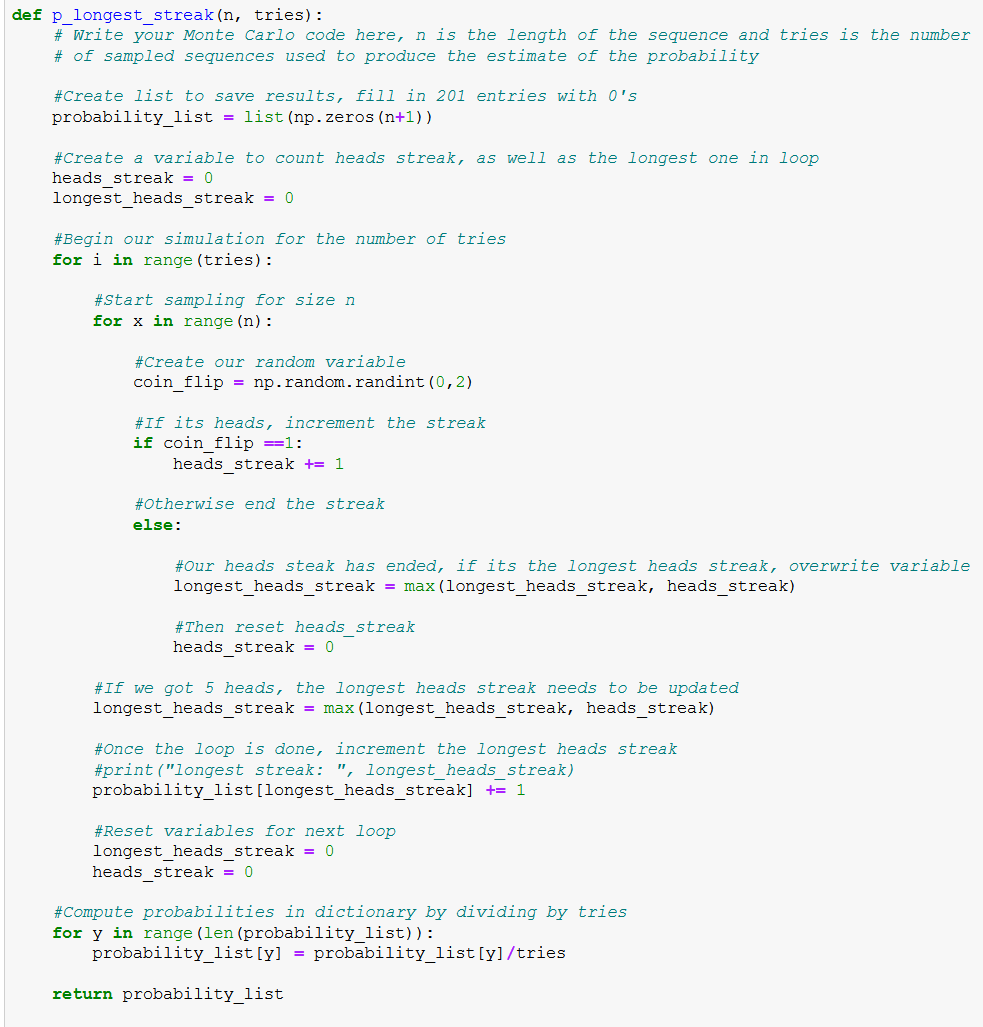
\includegraphics[scale=.5]{streaks screenshot.png} \\
 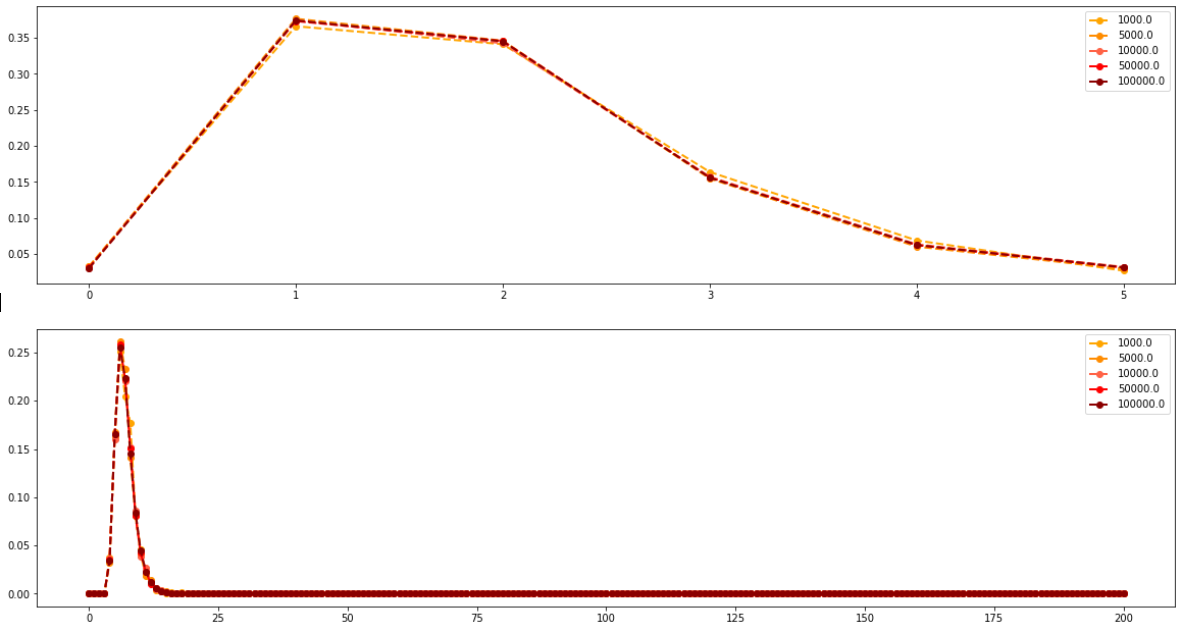
\includegraphics[scale=.5]{graphs for streaks.png}\\   

\end{document}
